\documentclass[10pt]{beamer}
\usetheme{Madrid}
\setbeamercovered{dynamic}
\usecolortheme{beaver}
% beaver è un tema grigio-rosso, ma non cambia il colore dei bullet di itemize e
% di enumerate.  Il seguente comando serve impostarli al colore darkred definito
% nel tema beaver.
\setbeamercolor{local structure}{fg=darkred}

\usepackage[T1]{fontenc}
\usefonttheme{professionalfonts}
\usepackage[sfmath,slantedGreeks]{kpfonts}
\usepackage[utf8]{inputenc}
\usepackage[italian]{babel}

\usepackage[beamer,customcolors]{hf-tikz}
\usepackage[autostyle=true]{csquotes}
\usepackage[backend=biber]{biblatex}
% purtroppo sembra che `particlessymb' serva a poco perché `hepparticles' non
% funziona granché bene in un contesto sans serif (anche se dice che dovrebbe
% riconoscerlo...), tutte le particelle con simboli latini devo usarle con cose
% del tipo `\textup', `\mathsf' (in contesto matematico), i comandi di
% `particlessymb' sono utili solo per le poche particelle con simboli greci
\usepackage{booktabs,graphicx,particlessymb,pifont,siunitx}
\usepackage[font=scriptsize,labelformat=empty]{caption}

\definecolor{darkblue}{rgb}{0,0,0.8}
\DeclareSIUnit\parsec{pc}
\DeclareSIUnit\clight{\text{\ensuremath{c}}}
\sisetup{per-mode=symbol,
  inter-unit-separator={}\cdot{},
  exponent-product=\cdot,
  output-product=\cdot,
  separate-uncertainty=true
}
\addbibresource{bibliografia.bib}

\DeclareMathOperator{\e}{\mathrm{e}}
\renewcommand{\phi}{\varphi}
\renewcommand{\epsilon}{\varepsilon}

\newcommand*{\dd}{\mathop{}\!\textup{d}} % Operatore differenziale \dd
% Derivata totale: \toder[ordine]{funzione}{variabile}
\newcommand*{\toder}[3][]{\frac{{\dd^{#1}}#2}{\dd {#3}^{#1}}}

% Simboli che si possono utilizzare negli elenchi dell'ambiente itemize.  `\pro'
% (nel senso di "vantaggio") produce un tick, `\con' (nel senso di "contro")
% produce un cross.  Usa simboli del pacchetto `pifont'
\newcommand{\pro}{\color{alerted text.fg}{\ding{51}}}
\newcommand{\con}{\color{alerted text.fg}{\ding{55}}}

\title[Recenti progressi sullo studio dei raggi cosmici (GeV)]{Recenti progressi
  sullo studio \\ dei raggi cosmici \\ nell'energia del GeV}
\author{Mosè Giordano}
\date{6 maggio 2013}
\institute{Università del Salento}
\titlegraphic{
\includegraphics[width=20mm]{logo-unisalento}}

\begin{document}
\begin{frame}
  \maketitle
\end{frame}

\begin{frame}
  \frametitle{Piano della presentazione}
  \tableofcontents
\end{frame}

\section{Introduzione}

% \subsection{I raggi cosmici}

% Per l'introduzione vedi l'articolo arXiv:1302.3307 e
% http://arstechnica.com/science/2013/02/supernova-observations-solve-the-mystery-of-cosmic-ray-origins/
% (questo può essere carino per l'inizio, parla della OMG particle)
\begin{frame}
  \frametitle{Raggi cosmici}
  I \alert{raggi cosmici} sono \alert{particelle cariche di alta energia} che
  viaggiano nell'Universo.  Composizione nella parte alta dell'atmosfera (per
  energia dell'ordine del \si{\giga\electronvolt})
  \begin{itemize}
  \item 79\% protoni
  \item 15\% \PGa
  \item 5\% nuclei più pesanti
  \item 1\% elettroni liberi
  \item \numrange[range-phrase=--]{e-5}{e-4} antiprotoni
  \end{itemize}
  Distribuzione sostanzialmente isotropa
\end{frame}

\begin{frame}
  \frametitle{Raggi cosmici: lo spettro energetico}
  \begin{columns}
    \begin{column}{0.55\columnwidth}
      Osservazione
      \begin{itemize}
      \item diretta (palloni e satelliti) per
        $E < \SIrange[range-phrase=-]{e12}{e14}{\electronvolt}$
      \item indiretta (sciami estesi in atmosfera) per
        $E > \SIrange[range-phrase=-]{e12}{e14}{\electronvolt}$
      \end{itemize}
      Flussi
      \begin{itemize}
      \item $E \sim \SI{e15}{\electronvolt}$:
        \SI{1}{particella\per\metre\squared\per anno}
      \item $E \sim \SI{e18}{\electronvolt}$:
        \SI{1}{particella\per\kilo\metre\squared\per anno}
      \item $E \sim \SI{e20}{\electronvolt}$:
        \SI{1}{particella\per\kilo\metre\squared\per secolo}
      \end{itemize}
    \end{column}
    \begin{column}{0.45\columnwidth}
      \begin{figure}
        \centering
        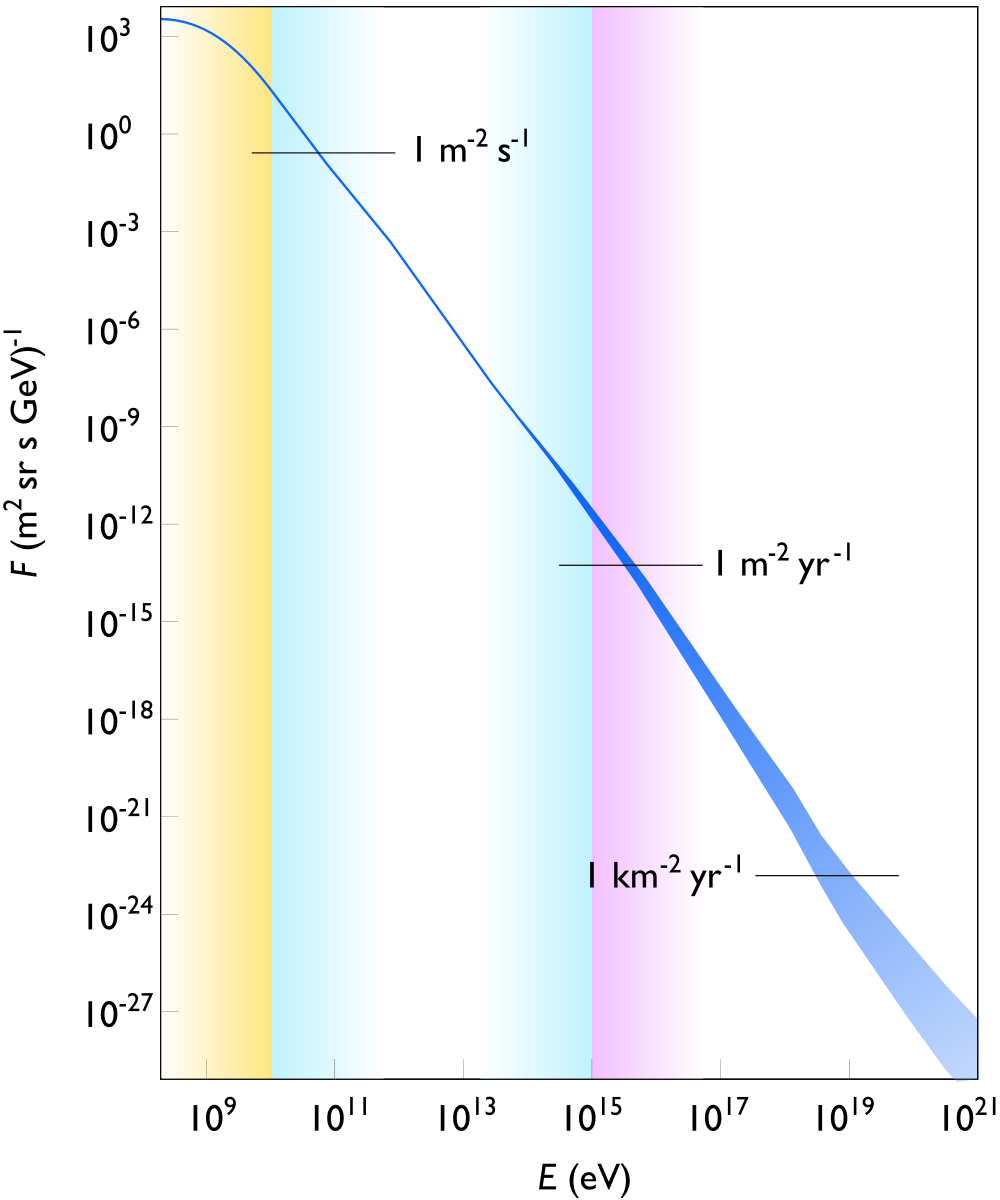
\includegraphics[width=\columnwidth]{cr-spectrum}
        \caption{Credit: Sven Lafebre}
      \end{figure}
    \end{column}
  \end{columns}
\end{frame}

\begin{frame}
  \frametitle{Raggi gamma}
  Possibili sorgenti di raggi gamma nelle SNR
  \begin{itemize}
  \item<+-> adronica, decadimento di \PGpz:
    \begin{equation*}
      \mathsf{p} + \mathsf{p} \to \PGpz + \mathsf{X}, \quad \PGpz \to 2\PGg
    \end{equation*}
  \item<+-> leptonica
    \begin{itemize}
    \item bremsstrahlung
    \item effetto Compton inverso
    \end{itemize}
  \end{itemize}
\end{frame}


\begin{frame}
  \frametitle{Positroni}
  % Discussione teorica presa da doi:10.1038/nature07942
  Una piccola parte dei raggi cosmici è costituita da antiparticelle, le quali
  sono prodotte dall'interazione fra i nuclei presenti nei raggi cosmici e gli
  atomi del mezzo interstellare (\alert{sorgente secondaria}).

  I positroni possono anche essere prodotti in pulsar o microquasars attraverso
  l'annichilazione di materia oscura (\alert{sorgente primaria}).

  Si ritiene che i protoni siano
  \alert{prodotti soprattutto da sorgenti secondarie}.

  Prendendo in considerazione le perdite di energia dei raggi cosmici primari,
  ci si aspetta che gli elettroni abbiano uno spettro più ``duro'' rispetto ai
  positroni, se questi sono soprattutto di origine secondaria.  Se quest'ultima
  ipotesi fosse valida,
  \alert{la frazione di positroni dovrebbe diminuire all'aumentare
    dell'energia}.
\end{frame}

\section{Risultati recenti}

\subsection{Fermi Gamma-ray Space Telescope}

\begin{frame}
  \frametitle{Fermi: l'esperimento}
  \begin{figure}
    \centering
    % Fonte:
    % http://commons.wikimedia.org/wiki/File:Diagram_of_the_GLAST_instrument.jpg
    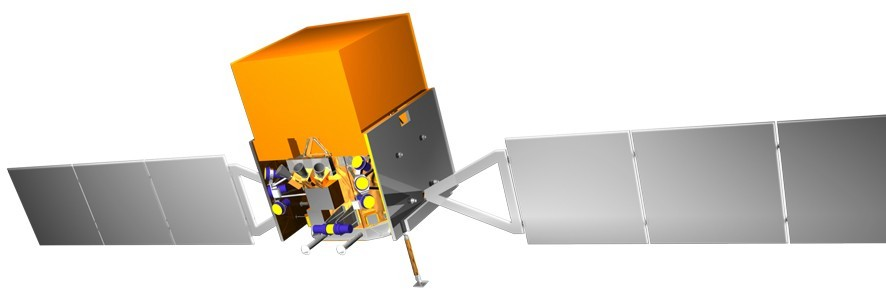
\includegraphics[width=0.5\columnwidth]{glast.jpg}
  \end{figure}
  Osservatorio per lo studio dei raggi gamma (da \SI{8}{\kilo\electronvolt} fino
  a oltre \SI{300}{\giga\electronvolt}) emessi da corpi celesti.  Obiettivi
  dell'esperimento:
  \begin{itemize}
  \item comprensione \alert{meccanismo di accelerazione particelle} in AGN,
    pulsar e SNR
  \item studio \alert{sorgenti gamma non identificate} e
    \alert{radiazione gamma diffusa} galattica ed extra-galattica
  \item studio \alert{emissione ad altissima energia} nei GRB
  \item rivelazione indiretta della \alert{materia oscura}, attraverso suo
    decadimento o annichilazione in fotoni o elettroni e positroni
  \item osservazione \alert{evaporazione di MBH} dalla presunta traccia di lampi
    gamma
  \end{itemize}
  È in orbita a \SI{550}{\kilo\metre} d'altezza dall'11 giugno 2008
\end{frame}

\begin{frame}
  \frametitle{Fermi: strumentazione}
  % Per approfondire vedi
  % http://www.nasa.gov/mission_pages/GLAST/spacecraft/index.html
  \begin{columns}
    \begin{column}{0.4\columnwidth}
      \begin{itemize}
      \item \alert{Large Area Telescope} (LAT), sensibile a singoli raggi gamma
        con energia tra \SI{20}{\mega\electronvolt} e
        \SI{300}{\giga\electronvolt}
      \item \alert{Gamma-Ray Burst Monitor} (GBM), studio di fenomeni transienti
        (GRB e brillamenti) a energie relativamente più basse (tra
        \SI{8}{\kilo\electronvolt} e \SI{40}{\mega\electronvolt})
      \end{itemize}
    \end{column}
    \begin{column}{0.6\columnwidth}
      \begin{figure}
        \centering
        % Fonte: http://commons.wikimedia.org/wiki/File:GLAST_schematic.jpg
        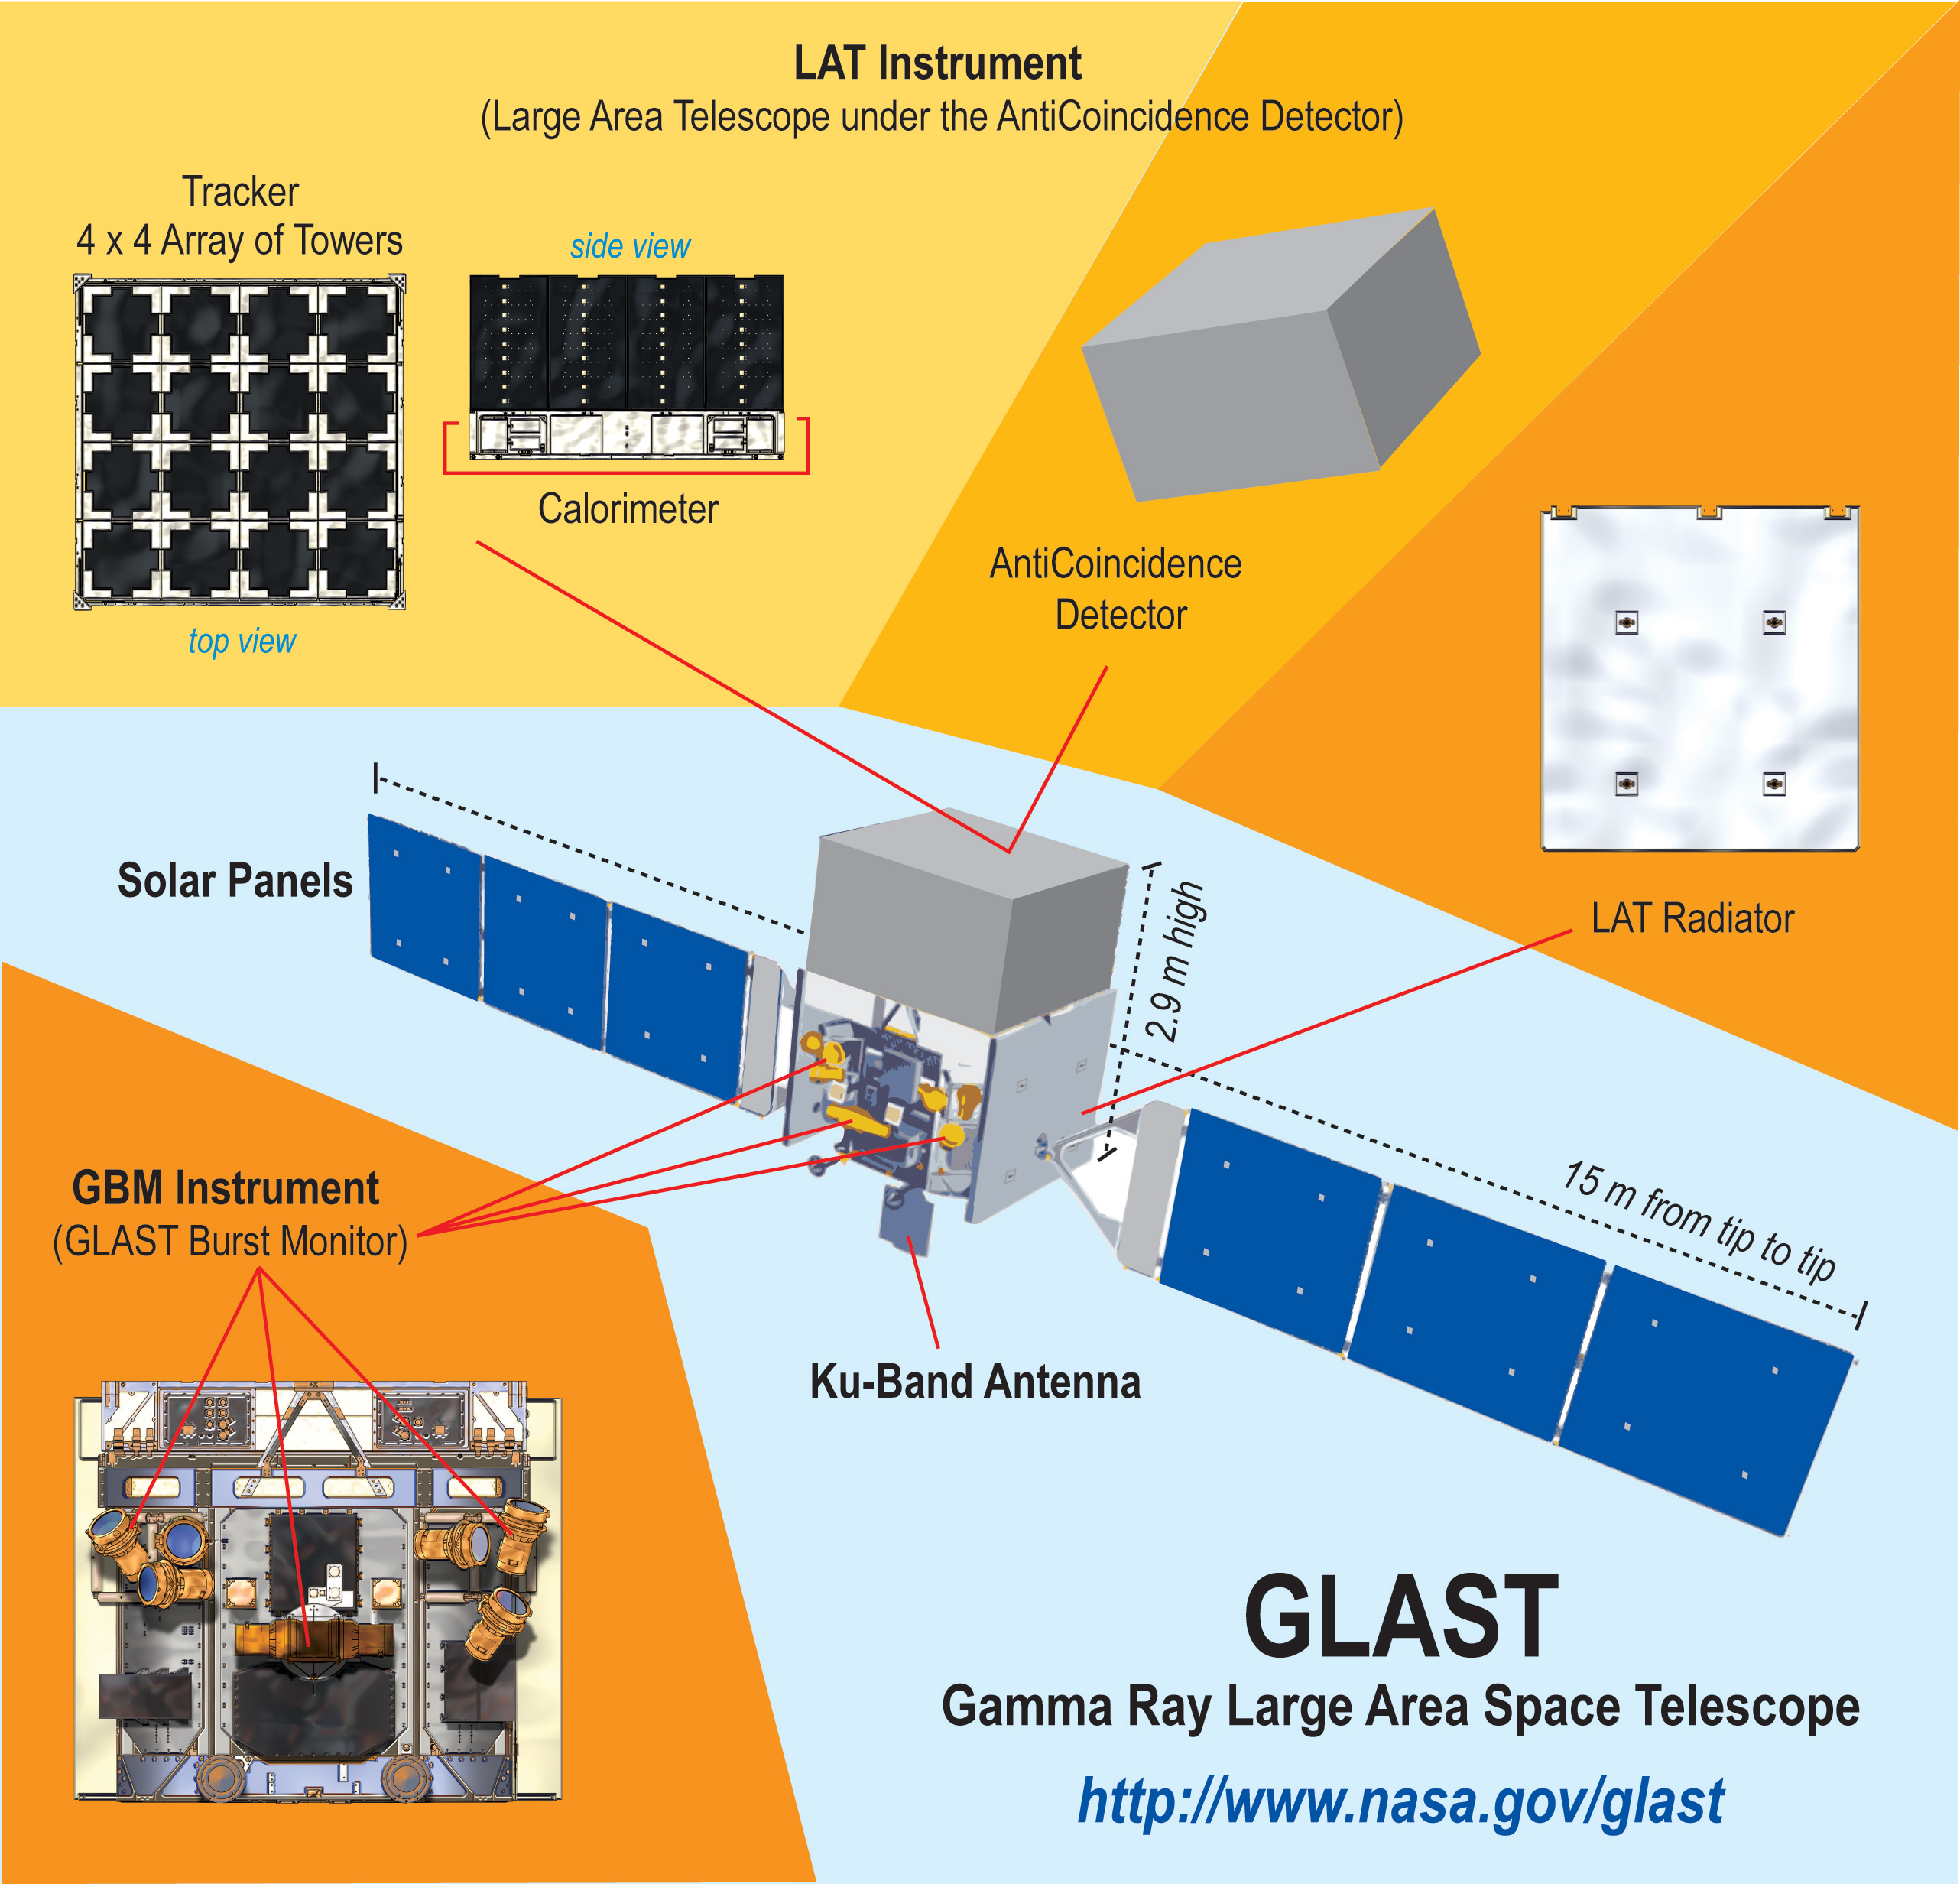
\includegraphics[width=\columnwidth]{glast_schematic.jpg}
      \end{figure}
    \end{column}
  \end{columns}
\end{frame}

\begin{frame}
  \frametitle{Fermi: LAT}
  % Importante: eliminazione del rumore costituito da raggi cosmici, vedi
  % sito indicato sopra.  Vedi anche
  % http://www-glast.stanford.edu/instrument.html
  \begin{figure}
    \centering
    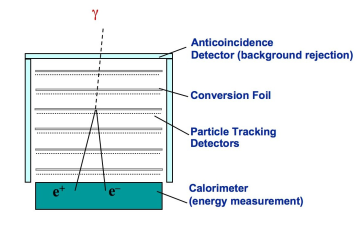
\includegraphics[width=0.6\columnwidth]{Gamma_telescope_schematic}
    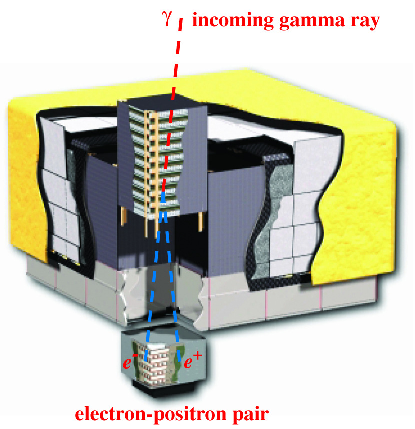
\includegraphics[width=0.4\columnwidth]{f1}
    \caption{Credit: \url{http://www-glast.stanford.edu/instrument.html}}
  \end{figure}
\end{frame}

\begin{frame}
  \frametitle{Fermi: SNR osservate}
  \begin{figure}
    \centering
    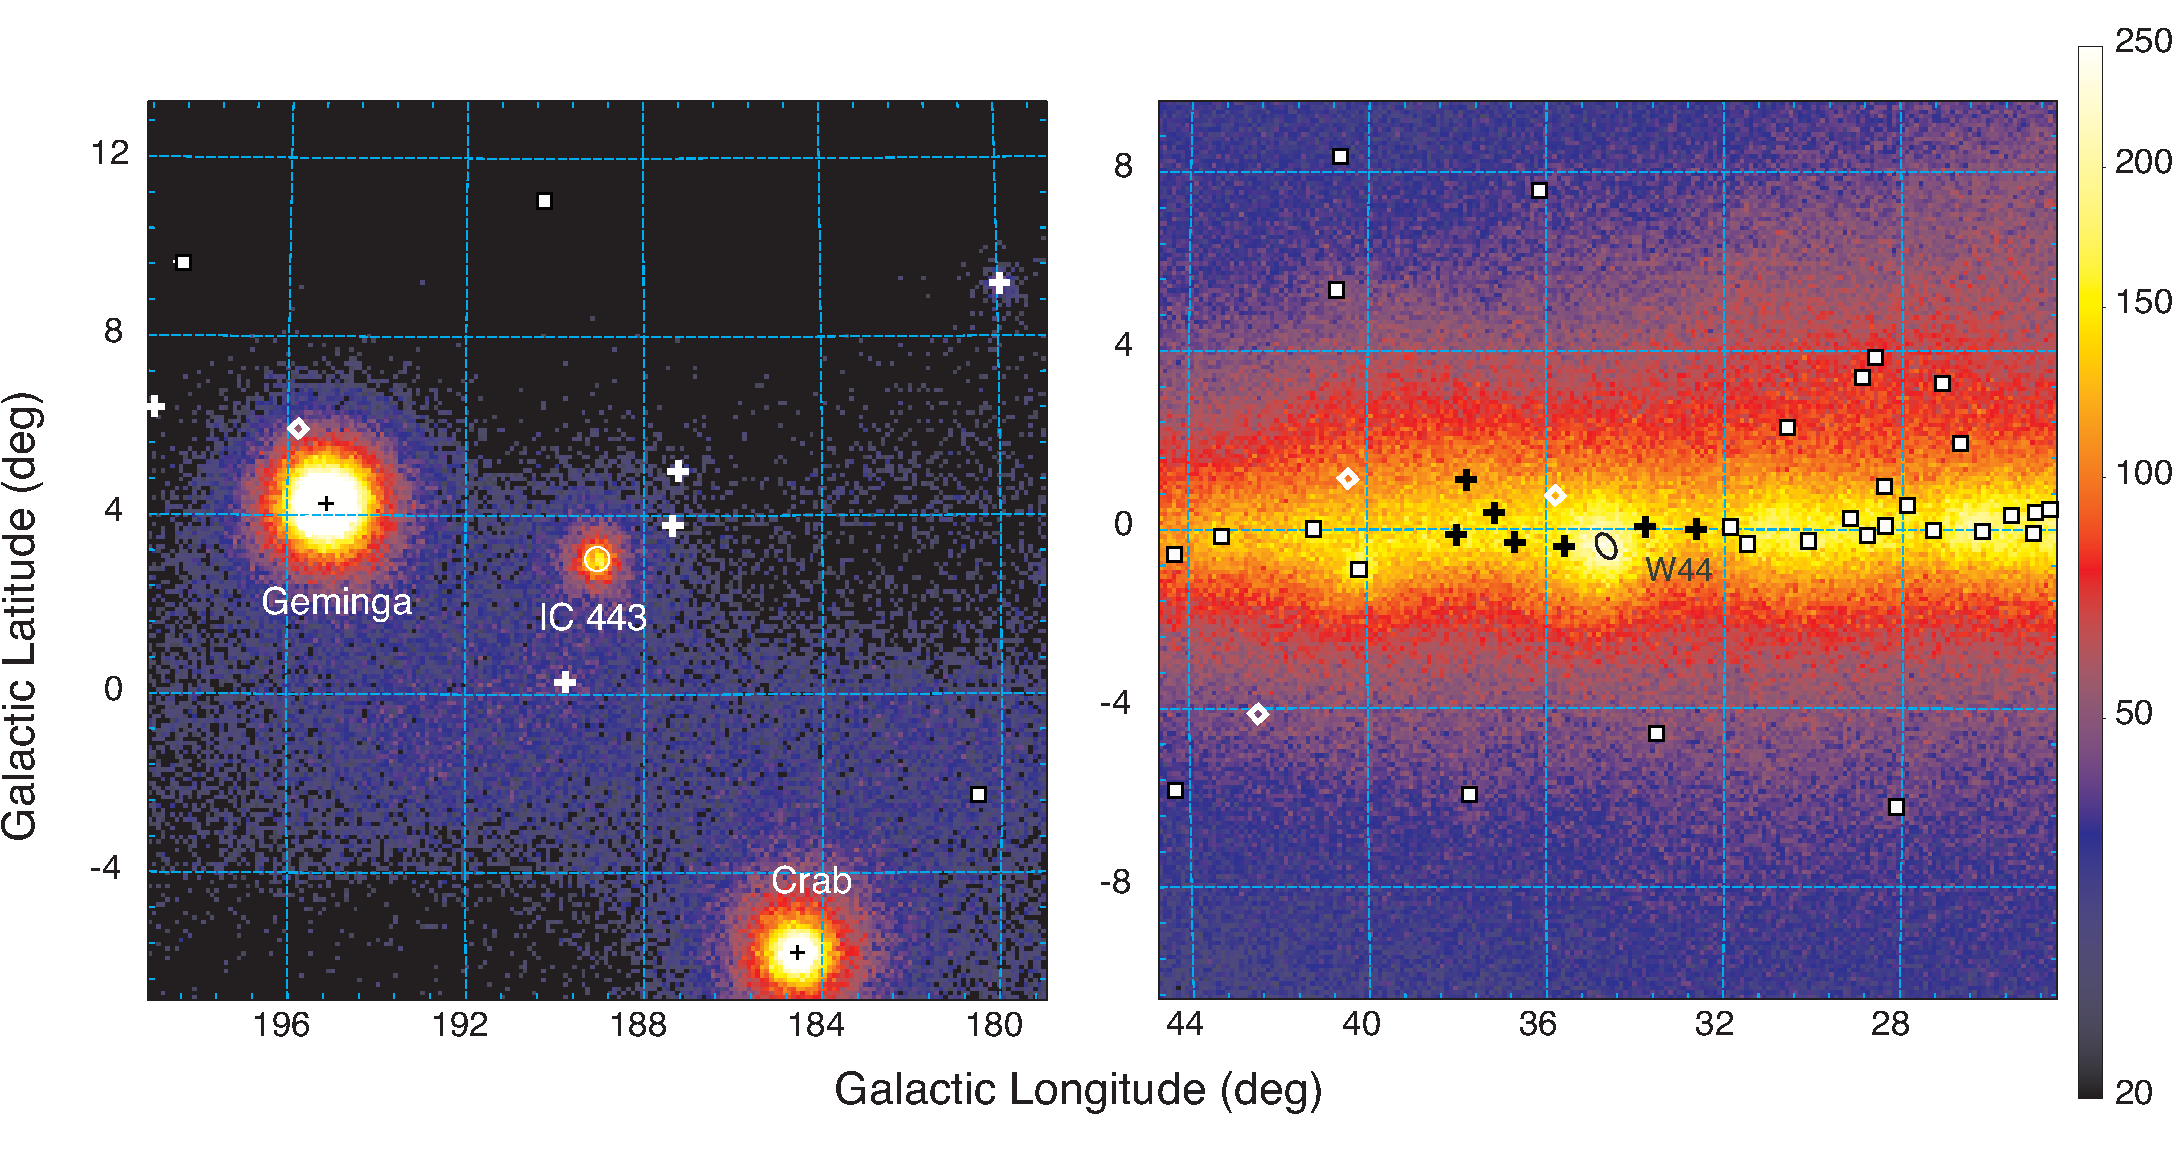
\includegraphics[width=0.8\columnwidth]{1231160fig1.pdf}
    \caption{Mappa del conteggio di raggi gamma in un campo di
      $\SI{20}{\degree} \times \SI{20}{\degree}$ attorno a IC 443 (sinistra,
      \SI{1.5}{\kilo \parsec}) e W44 (destra, \SI{2.9}{\kilo \parsec})
      nell'intervallo di energia da \SI{60}{\mega\electronvolt} a
      \SI{2}{\giga\electronvolt}.  Quadrati e croci indicano sorgenti gamma
      vicine, i rombi sorgenti precedentemente sconosciute.  Credit:
      \textcite{2013Sci...339..807A}}
  \end{figure}
\end{frame}

\begin{frame}
  \frametitle{Fermi-LAT: analisi dei dati}
  \begin{figure}
    \centering
    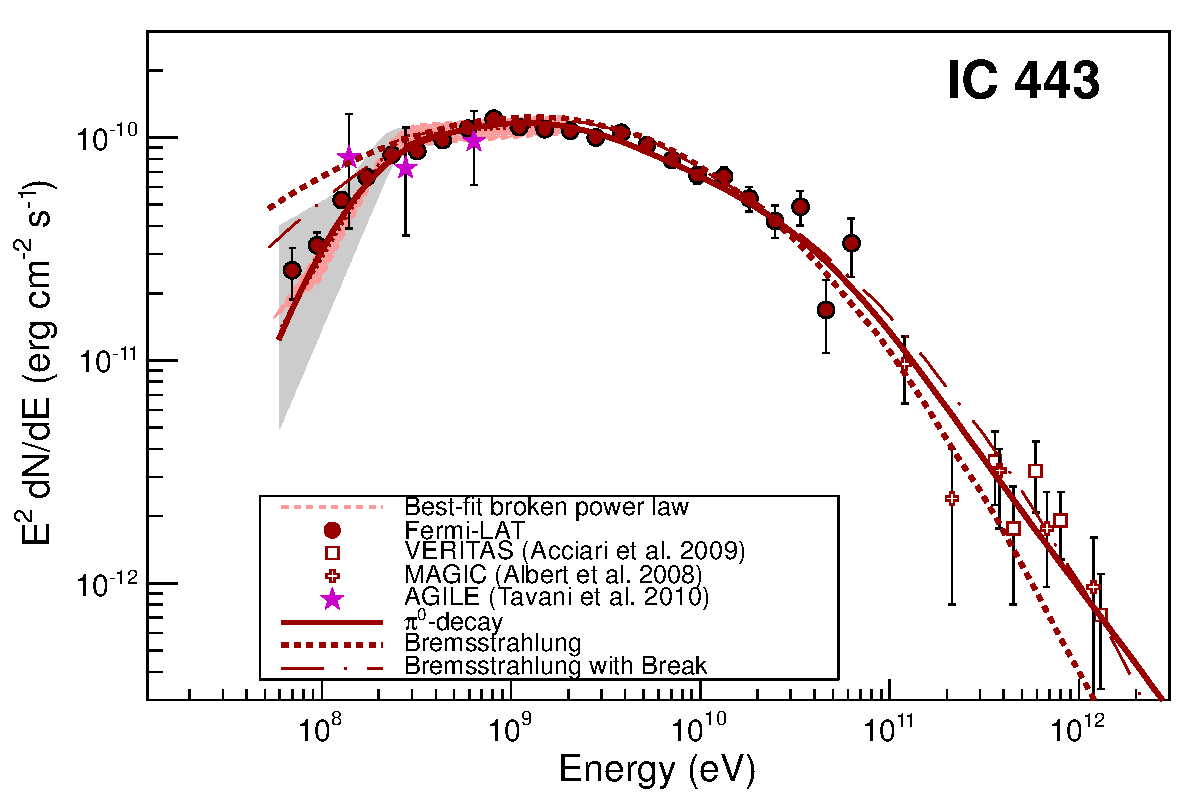
\includegraphics[width=0.5\columnwidth]{1231160fig2a}
    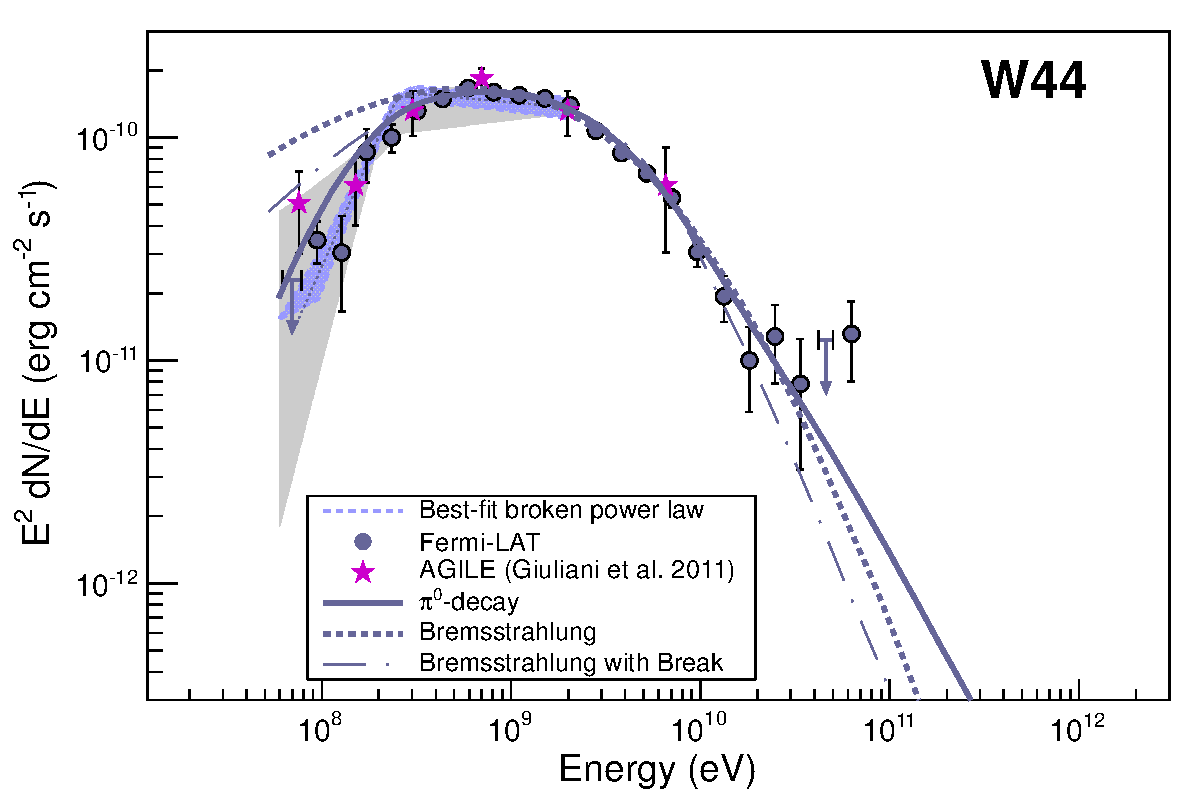
\includegraphics[width=0.5\columnwidth]{1231160fig2b}
    \caption{Spettro dei raggi gamma di IC 433 e W44, misurato da Fermi-LAT.
      Credit: \textcite{2013Sci...339..807A}}
  \end{figure}
\end{frame}

\begin{frame}
  \frametitle{Fermi-LAT: analisi dei dati (cont.)}
  Power law (PL):
  \begin{equation*}
    F(\epsilon) = K
    \left(
      \frac{\epsilon}{\epsilon_{0}}
    \right)^{-\Gamma_{1}}
  \end{equation*}
  Smoothly broken power law (BPL):
  \begin{equation*}
    F(\epsilon) = K
    \left(
      \frac{\epsilon}{\epsilon_{0}}
    \right)^{-\Gamma_{1}}
    \left(
      1 +
      \left(
        \frac{\epsilon}{\epsilon_{\textup{br}}}
      \right)^{(\Gamma_{2} - \Gamma_{1})/\alpha}
    \right)^{-\alpha}
  \end{equation*}
  $\epsilon_{0} = \SI{200}{\mega \electronvolt}$, parametro di smoothness del
  break fissato a $\alpha = 0.1$
  \begin{table}
    \centering
    %\sisetup{per-mode=reciprocal}
    \resizebox{\columnwidth}{!}{\begin{tabular}{cccccc}
        \toprule
        Modello & $K$ (cm\ap{$2$}s\ap{$-1$}MeV\ap{$-1$})
        & $\Gamma_1$ & $\Gamma_2$ & $\varepsilon_{\textup{br}}$
        (\si{\mega \electronvolt}) & $TS$ \\
        \midrule
        IC~443 & & & & & \\
        PL & $(11.7 \pm 0.2) \times 10^{-10}$ & $1.76\pm 0.02$
        & $\cdots$ & $\cdots$  &  21651 \\
        BPL & $(11.9 \pm 0.6) \times 10^{-10}$ & $0.57\pm 0.25$
        & $1.95^{+0.02}_{-0.02}$ & $245^{+16}_{-15}$  &  22010\\
        \midrule
        W44 & & & & & \\
        PL & $(13.0 \pm 0.4) \times 10^{-10}$ & $1.71\pm 0.03$
        & $\cdots$ & $\cdots$  &  6920 \\
        BPL & $(15.8 \pm 1.0) \times 10^{-10}$ & $0.07\pm 0.4$
        & $2.08^{+0.03}_{-0.03}$ & $253^{+11}_{-11}$  &  7351 \\
      \bottomrule
    \end{tabular}}
  \end{table}
\end{frame}

\begin{frame}
  \frametitle{Fermi-LAT: analisi dei dati (cont.)}
  \begin{figure}
    \centering
    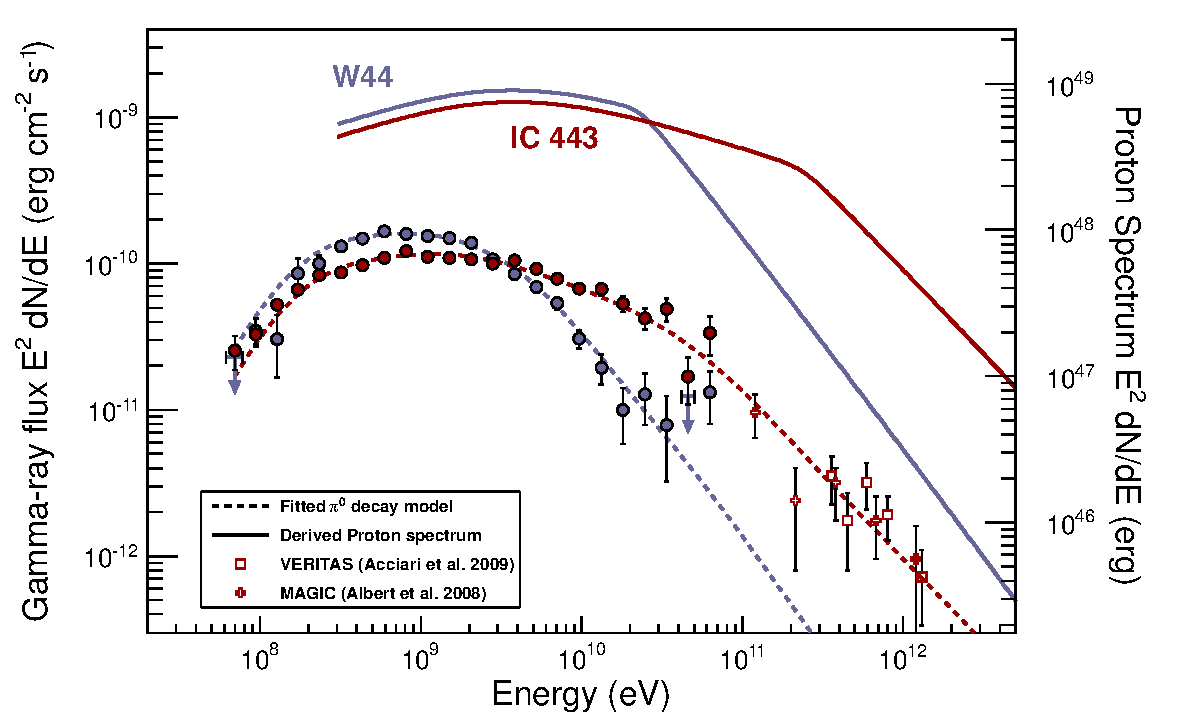
\includegraphics[width=.8\columnwidth]{1231160fig3}
    \caption{Spettro dei raggi gamma e dei protoni progenitori, derivato dallo
      spettro dei raggi gamma.  Credit: \textcite{2013Sci...339..807A}}
  \end{figure}
\end{frame}

\begin{frame}
  \frametitle{Fermi-LAT: analisi dei dati (cont.)}
  Lo spettro dei supposti protoni progenitori è stato derivato da una BPL della
  forma
  \begin{equation*}
    \toder{N_{\textup{p}}}{p} \propto
    \left(
      1 +
      \left(
        \frac{p}{p_{\textup{br}}}
      \right)^{(s_{1} - s_{2})/\beta}
    \right)^{-\beta}
  \end{equation*}
  Per IC~443: $s_{1} = \num{2.36(2)}$, $s_{2} = \num{3.1(1)}$,
  $p_{\textup{br}} = \SI{239(74)}{\giga \electronvolt \per \clight}$.  \\
  Per W44: $s_{1} = \num{2.36(5)}$, $s_{2} = \num{3.5(3)}$,
  $p_{\textup{br}} = \SI{22(8)}{\giga \electronvolt \per \clight}$.
\end{frame}

\begin{frame}
  \frametitle{Fermi-LAT: conclusioni}
  Le misure dello spettro dei raggi gamma effettuate da Fermi-LAT mostrano la
  presenza di una \alert{caratteristica del decadimento di \PGpz} non
  compatibile con un meccanismo primario di produzione di raggi gamma da
  elettroni relativistici (bremsstrahlung o effetto Compton inverso).  Ciò può
  essere interpretato come una
  \alert{prova diretta della presenza di protoni accelerati} nelle SNR
\end{frame}

\subsection{Alpha Magnetic Spectrometer}

\begin{frame}
  \frametitle{AMS-02: l'esperimento}
  \begin{figure}
    \centering
    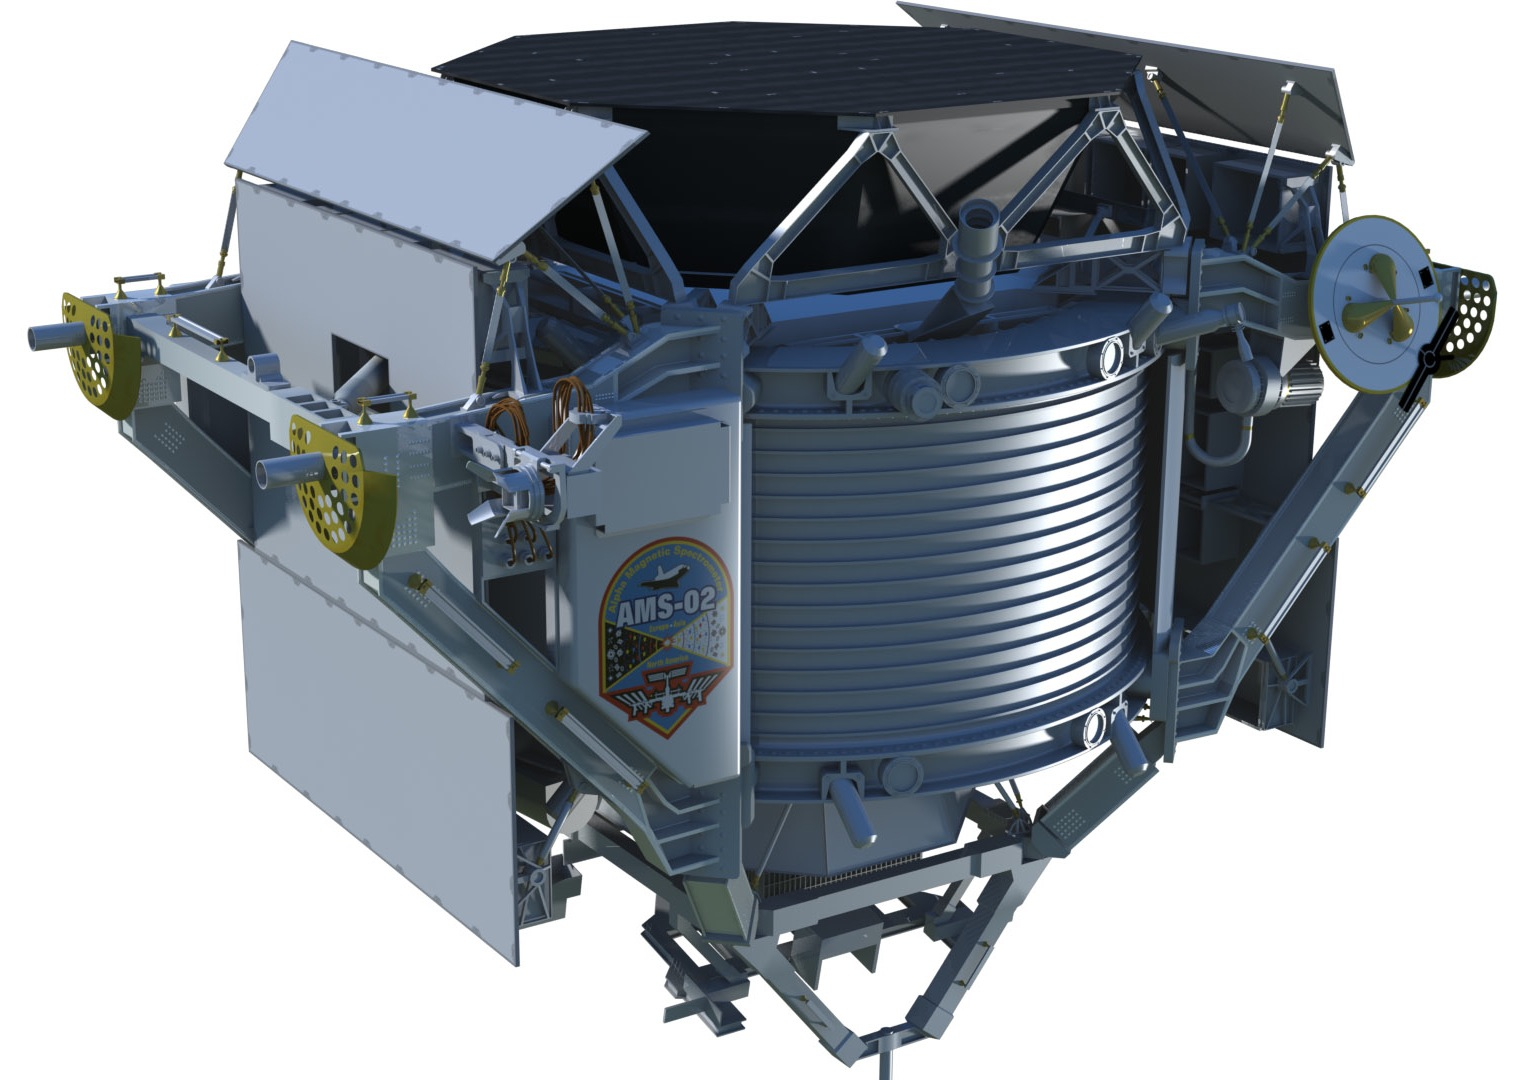
\includegraphics[width=0.3\columnwidth]{ams}
  \end{figure}
  È un modulo per condurre esperimenti di fisica delle particelle ad alte
  energie (\SIrange[range-phrase=--]{0.5}{350}{\giga\electronvolt}) installato
  sulla Stazione Spaziale Internazionale, a \SI{350}{\kilo\metre} di quota.
  Obiettivi dell'esperimento:
  \begin{itemize}
  \item analisi dei \alert{raggi cosmici}
  \item studi sulla \alert{formazione dell'Universo}
  \item ricerca di evidenze di \alert{materia oscura}
  \item studio dell'\alert{antimateria}
  \end{itemize}
  È stato montato a bordo della ISS il 19 maggio 2011
\end{frame}

\begin{frame}
  \frametitle{AMS-02: i rivelatori}
  \begin{figure}
    \centering
    % http://www.ams02.org/it/che-cosa-ams/strumenti/
    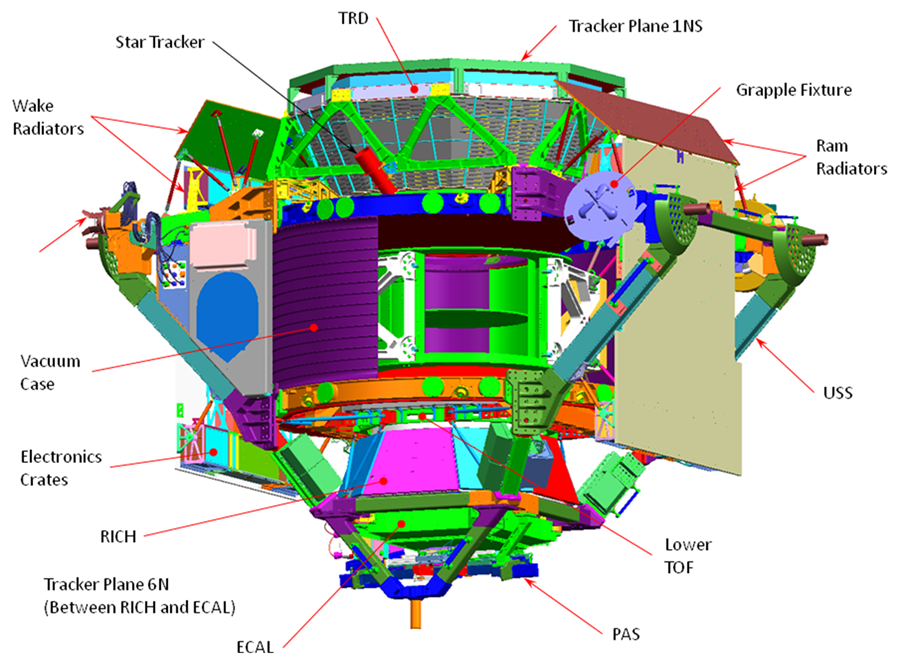
\includegraphics[width=.85\columnwidth]{ams-rivelatori}
  \end{figure}
\end{frame}

\begin{frame}
  \frametitle{AMS-02: i rivelatori (cont.)}
  \begin{figure}
    \centering
    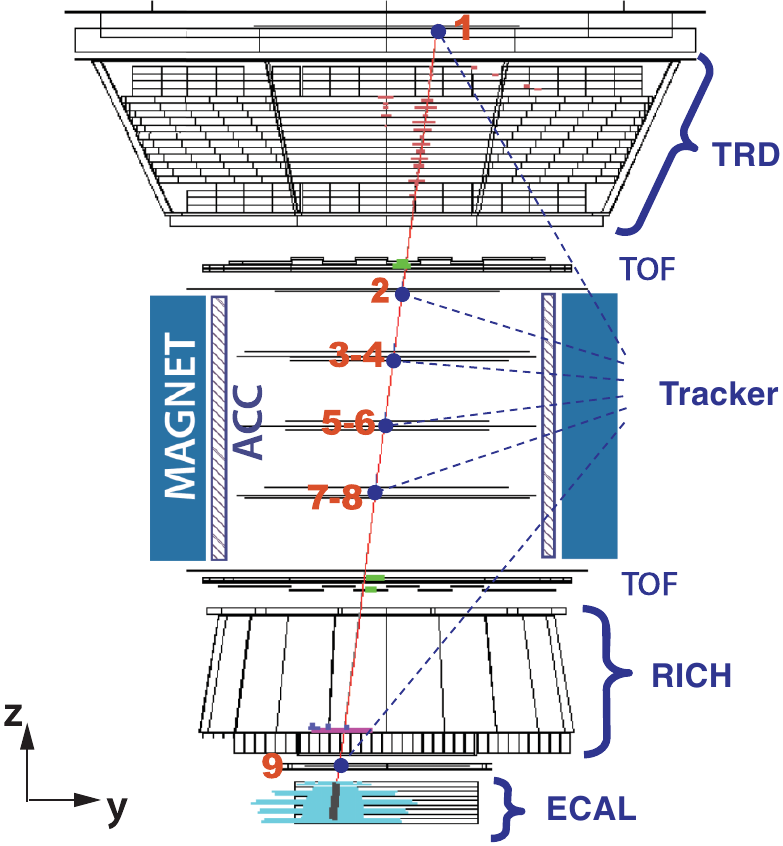
\includegraphics[width=.5\columnwidth]{ams-rivelatori2}
    \caption{Credit: \textcite{2013PhRvL.110n1102A}}
  \end{figure}
\end{frame}

\begin{frame}
  \frametitle{AMS-02: analisi dei dati}
  \begin{figure}
    \centering
    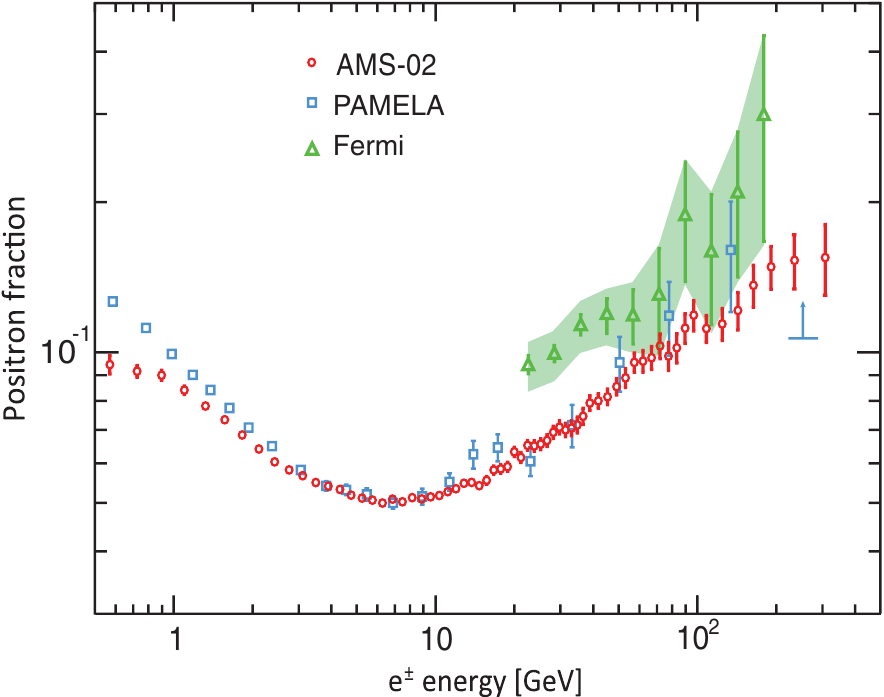
\includegraphics[width=.7\columnwidth]{ams1}
    \caption{Credit: \textcite{2013PhRvL.110n1102A}}
  \end{figure}
\end{frame}

\begin{frame}
  \frametitle{AMS-02: analisi dei dati (cont.)}
  Fit con un modello minimale.  Flussi di positroni ed elettroni
  \begin{gather*}
    \Phi_{\textup{e}^{+}} =
    \tikzmarkin<2>[set fill color=darkred!10,set border color=darkred]{a}
    C_{\textup{e}^{+}}E^{-\gamma_{\textup{e}^{+}}} \tikzmarkend{a} +
    \tikzmarkin<4>[set fill color=darkred!50!darkblue!10,set border
    color=darkred!50!darkblue]{b}C_{\textup{s}}E^{-\gamma_{\textup{s}}}
    \e^{-E/E_{\textup{s}}}\tikzmarkend{b} \\
    \Phi_{\textup{e}^{-}} =
    \tikzmarkin<3>[set fill color=darkblue!10,set border color=darkblue]{c}
    C_{\textup{e}^{-}}E^{-\gamma_{\textup{e}^{-}}} \tikzmarkend{c} +
    \tikzmarkin<4>[set fill color=darkred!50!darkblue!10,set border
    color=darkred!50!darkblue]{d}C_{\textup{s}}E^{-\gamma_{\textup{s}}}
    \e^{-E/E_{\textup{s}}}\tikzmarkend{d}
  \end{gather*}
  Frazione di positroni
  \begin{equation*}
    \frac{\Phi_{\textup{e}^{+}}}{\Phi_{\textup{e}^{+}} + \Phi_{\textup{e}^{-}}}
    = \frac{C_{\textup{e}^{+}}E^{-\gamma_{\textup{e}^{+}}} +
      C_{\textup{s}}E^{-\gamma_{\textup{s}}}
      \e^{-E/E_{\textup{s}}}}{C_{\textup{e}^{+}}E^{-\gamma_{\textup{e}^{+}}} +
      C_{\textup{e}^{-}}E^{-\gamma_{\textup{e}^{-}}} +
      2C_{\textup{s}}E^{-\gamma_{\textup{s}}}
      \e^{-E/E_{\textup{s}}}}
  \end{equation*}
\end{frame}

\begin{frame}
  \frametitle{AMS-02: analisi dei dati (cont.)}
  \begin{figure}
    \centering
    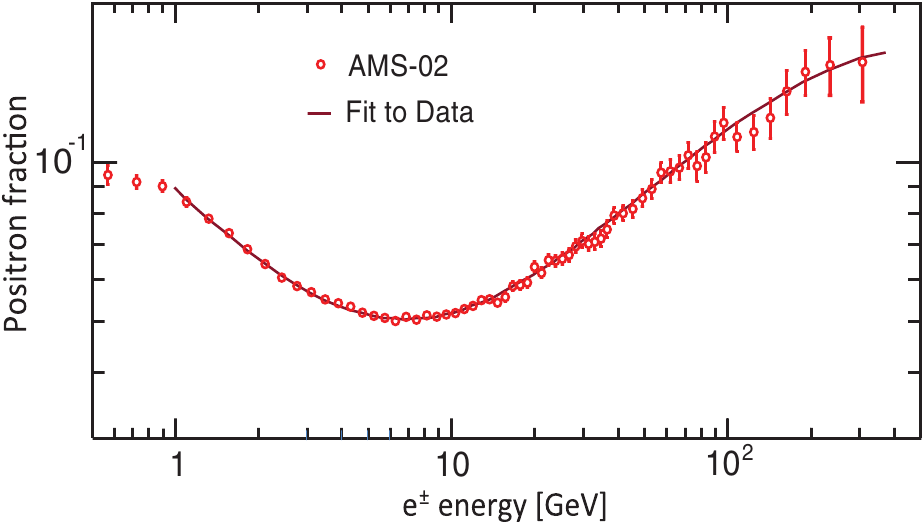
\includegraphics[width=.6\columnwidth]{ams2}
    \caption{Credit: \textcite{2013PhRvL.110n1102A}}
  \end{figure}
  $\gamma_{\textup{e}^{-}} - \gamma_{\textup{e}^{+}} = \num{-0.63(3)}$ \\
  $\gamma_{\textup{e}^{-}} - \gamma_{\textup{s}} = \num{0.66(5)}$ \\
  $C_{\textup{e}^{+}}/C_{\textup{e}^{-}} = \num{0.091(1)}$ \\
  $C_{\textup{s}}/C_{\textup{e}^{-}} = \num{0.0078(12)}$ \\
  $1/E_{\textup{s}} =
  \SI[per-mode=reciprocal]{0.0013(7)}{\per\giga\electronvolt} \implies
  E_{\textup{s}} = 760^{+1000}_{-280} \si{\giga \electronvolt}$ \\
  $\chi^{2}/\text{d.f.} = 28.5/57$
\end{frame}

\begin{frame}
  \frametitle{AMS-02: analisi dei dati (cont.)}
  Fluttuazioni della frazione osservata di positroni
  \begin{equation*}
    \frac{r_{\Pe}(b,l)}{\langle r_{\Pe}\rangle} - 1 = \sum_{\ell=0}^{\infty}
    \sum_{m=-\ell}^{\ell} a_{\ell m}Y_{\ell}^{m}(\pi/2 - b,l)
  \end{equation*}
  Coefficienti dello spettro di potenza angolare
  \begin{equation*}
    C_{\ell} = \frac{1}{2\ell + 1} \sum_{m=-\ell}^{\ell} \lvert a_{\ell m}
    \rvert^{2}
  \end{equation*}
  Ampiezza dell'anisotropia di dipolo
  \begin{equation*}
    \delta = 3 \sqrt{\frac{C_{1}}{4\pi}} \leq 0.036 \qquad (95\% \text{ CL})
  \end{equation*}
\end{frame}

\begin{frame}
  \frametitle{AMS-02: conclusioni}
  Questi primi dati raccolti da AMS-02 mostrano
  \begin{enumerate}[<+->]
  \item fino a \SI{10}{\giga \electronvolt}, una
    \alert{decrescita della frazione di positroni} all'aumentare dell'energia
  \item un evidente \alert{aumento della frazione di positroni} da
    \SIrange[range-phrase={ fino a }]{10}{\sim 250}{\giga \electronvolt}
  \item che la determinazione del comportamento della frazione di positroni fra
    \SIrange[range-phrase={ e }]{250}{350}{\giga \electronvolt} richiede una
    \alert{maggiore statistica}
  \item che la
    \alert{pendenza della frazione di positroni in funzione dell'energia
      diminuisce}
    di un ordine di grandezza da
    \SIrange[range-phrase={ a }]{20}{250}{\giga \electronvolt} e non si osserva
    \alert{nessuna struttura fine}
  \item il rapporto positroni/elettroni è compatibile con l'ipotesi di isotropia
  \end{enumerate}
  \uncover<+->{L'ipotesi di \alert{sola sorgente secondaria non è sufficiente}
    per spiegare l'aumento della frazione di positroni, è necessario invocare un
    \alert{altro fenomeno}, di fisica delle particelle o altra sorgente
    astrofisica}
\end{frame}

\begin{frame}
  \frametitle{AMS-02: conclusioni (cont.)}
  Possibili spiegazioni dell'aumento della frazione di positroni
  \begin{itemize}
  \item<+-> pulsar
  \item<+-> materia oscura
    \begin{itemize}
    \item[\con] distribuzione isotropa
    \item[\con] spettro dovrebbe presentare un picco intorno a metà della massa
      della particella originaria (e.g., neutralino) se decade in e\ap{+} +
      e\ap{-}
    \end{itemize}
  \end{itemize}
\end{frame}

\section{\refname}

\begin{frame}
  \frametitle{\refname{}}
  \printbibliography{}
\end{frame}
\end{document}

%%% Local Variables:
%%% mode: latex
%%% TeX-master: t
%%% End:
